\documentclass[
  a4paper,
  12pt,
  spanish,
]{scrartcl}

% Párrafos
\setlength{\parindent}{18pt}
\linespread{1.05}

%-------------------------------------------------------------------------------
%	PAQUETES
%-------------------------------------------------------------------------------

% Idioma

\usepackage[es-noindentfirst]{babel}

% Citas de texto en línea/bloque

\usepackage[autostyle]{csquotes}

% Matemáticas

\usepackage{amsmath, amsthm, amssymb}
\usepackage{mathtools}
\usepackage{commath}

% Fuentes personalizadas para utilizar con XeLaTeX o LuaLaTeX

\usepackage[no-math]{fontspec}
\setmainfont{Libertinus Serif}
\setsansfont{Libertinus Sans}
\setmonofont[Scale=.9]{Libertinus Mono}

\usepackage[math-style=TeX]{unicode-math}
\setmathfont{Libertinus Math}

% Configuración de microtype

\defaultfontfeatures{Ligatures=TeX,Numbers=Lining}
\usepackage[activate={true,nocompatibility},final,tracking=true,factor=1100,stretch=10,shrink=10]{microtype}
\SetTracking{encoding={*}, shape=sc}{0}

% Enlaces y colores

\usepackage{hyperref}
\usepackage[dvipsnames]{xcolor}
\definecolor{webgreen}{rgb}{0,0.5,0}
\hypersetup{
  colorlinks=true,
  citecolor=webgreen,
  urlcolor=Maroon,
  linkcolor=RoyalBlue
}

% Otros elementos de página

\usepackage{enumitem}
\setlist[enumerate]{leftmargin=*, itemsep=0pt}
\setlist[itemize]{leftmargin=*, itemsep=0pt}

\usepackage[labelfont=sc]{caption}

% Tikz

\usepackage{tikz}
\usetikzlibrary{babel}
\usepackage{float}

% Código

\usepackage{listings}
\lstset{
	basicstyle=\footnotesize\ttfamily,%
	breaklines=true,%
	captionpos=b,                    % sets the caption-position to bottom
  tabsize=2,	                   % sets default tabsize to 2 spaces
  frame=lines,
  numbers=left,
  stepnumber=1,
  aboveskip=12pt,
  showstringspaces=false,
}
\renewcommand{\lstlistingname}{Listado}

\usepackage{fancyvrb}

% Bibliografía

\usepackage[sorting=none, style=apa, isbn=true]{biblatex}
\DefineBibliographyStrings{spanish}{
  urlseen = {Consultado},
  retrieved = {Consultado},
}
\addbibresource{bibliografia.bib}

% Lorem ipsum

\usepackage{blindtext}

% Márgenes
\usepackage[bottom=3.125cm, top=2.5cm, left=4.5cm, right=4.5cm, marginparwidth=70pt]{geometry}

% Fuentes

\usepackage{textcase}

\newfontfamily{\sacshape}{Libertinus Serif}[
  WordSpace={1.8},
  LetterSpace={18.0}
]

\newfontfamily{\slscshape}{Libertinus Serif}[
  WordSpace={1.8},
  LetterSpace={6.0}
]

\DeclareRobustCommand{\spacedallcaps}[1]{{\linespread{1.3}\sacshape\MakeTextUppercase{#1}}}% WordSpace=1.8
\DeclareRobustCommand{\spacedlowsmallcaps}[1]{{\slscshape\MakeTextLowercase{#1}}}% WordSpace=1.8

% Cabeceras de sección

\RedeclareSectionCommands[beforeskip=-3ex,
afterskip=2ex]{section,subsection,subsubsection}
%\addtokomafont{section}{\normalfont\large\spacedallcaps}
%\setkomafont{section}{\normalfont\large\scshape}
\RedeclareSectionCommand[beforeskip=-9ex, font=\normalfont\large\scshape, tocentryformat=\normalfont\scshape]{section}
\addtokomafont{subsection}{\normalfont\normalsize\itshape}
\RedeclareSectionCommand[beforeskip=-6ex,tocentryformat=\normalfont\itshape]{subsection}
\addtokomafont{subsubsection}{\normalfont}
\RedeclareSectionCommand[beforeskip=-4ex]{subsubsection}
\addtokomafont{paragraph}{\normalfont\itshape}
%-------------------------------------------------------------------------------
%	TÍTULO
%-------------------------------------------------------------------------------

\newcommand{\horrule}[1]{\rule{\linewidth}{#1}}

%-------------------------------------------------------------------------------
%	CONTENIDO
%-------------------------------------------------------------------------------

\begin{document}

\begin{titlepage}
  \vspace*{4cm}

  \begin{flushleft}
    \Huge
    \spacedallcaps{Red Tor}
    \horrule{2pt}
  \end{flushleft}

  \vspace{2em}

  \begin{flushright}
    \large
    José María Martín Luque\\
    Antonio Martín Ruiz\\
    Daniel Pozo Escalona\vspace{1em}

    \textit{Seguridad y Protección de Sistemas Informáticos}

    Grado en Ingeniería Informática

    \textsc{Universidad de Granada}\vspace{1em}

    \today\vspace{.5em}
  \end{flushright}
\end{titlepage}

\newpage

{\hypersetup{hidelinks}
\tableofcontents
}

\newpage

\section{Introducción: ¿qué es Tor?}
% Común

Tor es una red superpuesta\footnote{
  Una red superpuesta es una red virtual de nodos enlazados lógicamente que utiliza la infraestructura de otra red existente \parencite[154]{kurose_computer_2013}.
} distribuida diseñada para anonimizar aplicaciones de baja latencia basadas en el protocolo TCP, como pueden ser un navegador web, una aplicación que implemente el protocolo SSH o un servicio de mensajería instantánea.
Los clientes escogen un camino a través de la red y crean un <<circuito>> en el que cada nodo ---o <<\textit{router} cebolla>>--- en dicho camino conoce su predecesor y sucesor pero no el resto de nodos del circuito.

En la sección \ref{sec:estructura} veremos cómo se estructura la red Tor, estudiando el funcionamiento de los nodos que la componen. 
Por otro lado, en la sección \ref{sec:enrutamiento} realizaremos una breve descripción de la técnica que permite el anonimato de la red Tor, el \textit{enrutamiento cebolla}. 
En la sección \ref{sec:algoritmos} veremos con algo más de detalle los algoritmos de cifrado que utiliza Tor y con qué parámetros. 
Finalmente, en la sección \ref{sec:ataques} mostraremos algunos de los posibles ataques que se pueden realizar sobre esta red.  

\section{Estructura de la red Tor}
\label{sec:estructura}

% Each user runs local software called an onion proxy (OP) to fetch directories, establish circuits across the network, and handle connections from user applications.

La red Tor está formada por nodos que se comunican mediante TLS/SSLv3 sobre TCP/IP para mantener íntegra y oculta la información entre comunicaciones. Los nodos reciben el tráfico y lo reenvían.

El tráfico pasa por, al menos, tres nodos antes de llegar a su destino. Según la función que cumplen los nodos dentro del circuito podemos diferenciar tres tipos:

\begin{itemize}
\item Nodos intermedios. Reciben el tráfico y lo pasan a otro nodo. La presencia de los nodos intermedios es pública para toda la red Tor y cualquier usuario puede conectarse a ellos.
\item Nodos salida. Nodo final por el cuál pasa el tráfico antes de alcanzar su destino. Son también de acceso público para toda la red tor. La IP de estos nodos es interpretada por el receptor de información como la fuente del tráfico.
\item Puentes (\textit{bridges}). Nodos que no son públicos en la red Tor. Utilizados para evitar medidas de censura en países en los que regularmente se bloquean las IP de todos los nodos listados públicamente. Realizan la misma función que los nodos intermedios.
\end {itemize}

Cada nodo almacena dos claves: una \textit{clave de identidad} duradera y una \textit{clave cebolla} efímera. La clave de identidad se utiliza para firmar los certificados TLS y para firmar el descriptor de dicho nodo, que contiene información como su dirección o ancho de banda. La clave cebolla se utiliza para descifrar las peticiones de los usuarios y negociar las claves efímeras.

Existe además un servicio de directorio que publica la lista de nodos disponibles e información sobre ellos. Esta información es accesible a todos los nodos intermedios y todos los usuarios finales la usan para poder conectarse a la red. Existen una serie de nodos principales llamados \textit{autoridades de directorio} ---nodos confiables--- y nodos secundarios que actúan como \textit{caché} y \textit{backup} de los principales. Para dar fiabilidad al servicio de directorio las entradas son protegidas mediante firmas y solo la información proveniente de autoridades de directorio aprobadas son publicadas en la base de datos. Todo nodo nuevo de la red debe ser previamente aprobado, no existiendo un procedimiento automático para ello. Los administradores del servicio de directorio deben hacerlo manualmente.

\section{Enrutamiento cebolla}
\label{sec:enrutamiento}
% Antonio

Para el envío de tráfico a través de la red se utiliza un procedimiento llamado \textit{enrutamiento cebolla}. Esto es debido a cómo se acumulan capas de cifrado sobre el mensaje original. Veamos el procedimiento general y en apartados posteriores desarrollaremos más ampliamente los procedimientos criptográficos utilizados.

El tráfico se envía en paquetes de un tamaño fijo de \(512\) bytes segmentados en dos partes, cabecera y datos. 
En la cabecera se almacena información de control, que permite indentificar el circuito al que se envía la información además del comando que describe qué hacer con los datos del paquete.
Existen en consecuencia dos tipos de paquetes: de control, que son interpretados por el nodo que los recibe, y de retransmisión, que deben ser redirigidos por el nodo al siguiente en el circuito.
Toda la información de los paquetes de retransmisión ---cabecera y datos--- está cifrada siendo descifrada conforme avanza en el circuito.

El usuario emisor consulta su propia configuración y el directorio de nodos para obtener la información sobre como formar el circuito. Selecciona entonces los nodos que pretende utilizar. Por defecto cada circuito tiene tres nodos intermedios.

Se negocian las claves de cifrado con cada nodo del circuito de forma individual, paso a paso. Se establecen claves simétricas efímeras mediante \textit{Diffie-Hellman} utilizando la clave cebolla del nodo. Mediante estas claves efímeras se cifra la información a intercambiar entre el usuario y el nodo. El circuito se construye desde el punto de partida, el usuario. Los mensajes para negociar las claves entre el nodo \(n\) y el \(n+1\) se realiza retransmitiendo paquetes entre el emisor y retransmitiendo paquetes desde el nodo \(1\) hasta el \(n\), y de ahí al nodo \(n+1\). En cada paso los mensajes son cifrados con las claves previamente negociadas. Una vez establecidas, se puede enviar tráfico. En la figura \ref{fig:or4} se puede observar gráficamente esta idea.

\begin{figure}[h]
  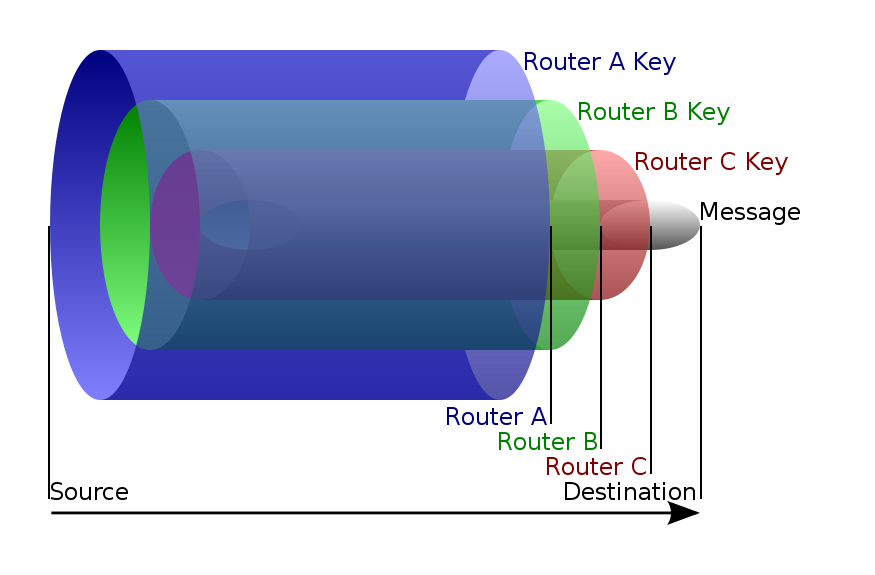
\includegraphics[width=\textwidth]{OR4.png}
  \caption{Representación visual del enrutamiento cebolla \parencite{wikipedia:hantwister_svg_2008}.}
  \label{fig:or4}
\end{figure}

Los paquetes se cifran con las claves recibidas en orden inverso: primero se cifra con la clave del último nodo, luego con la del penúltimo, y así hasta llegar al primero. Se envía el paquete resultante a través del circuito y a su paso por cada nodo se elimina la capa de cifrado correspondiente a dicho nodo. En la figura \ref{fig:or5} puede verse un esquema de un ejemplo de comunicación.

\begin{figure}[h]
  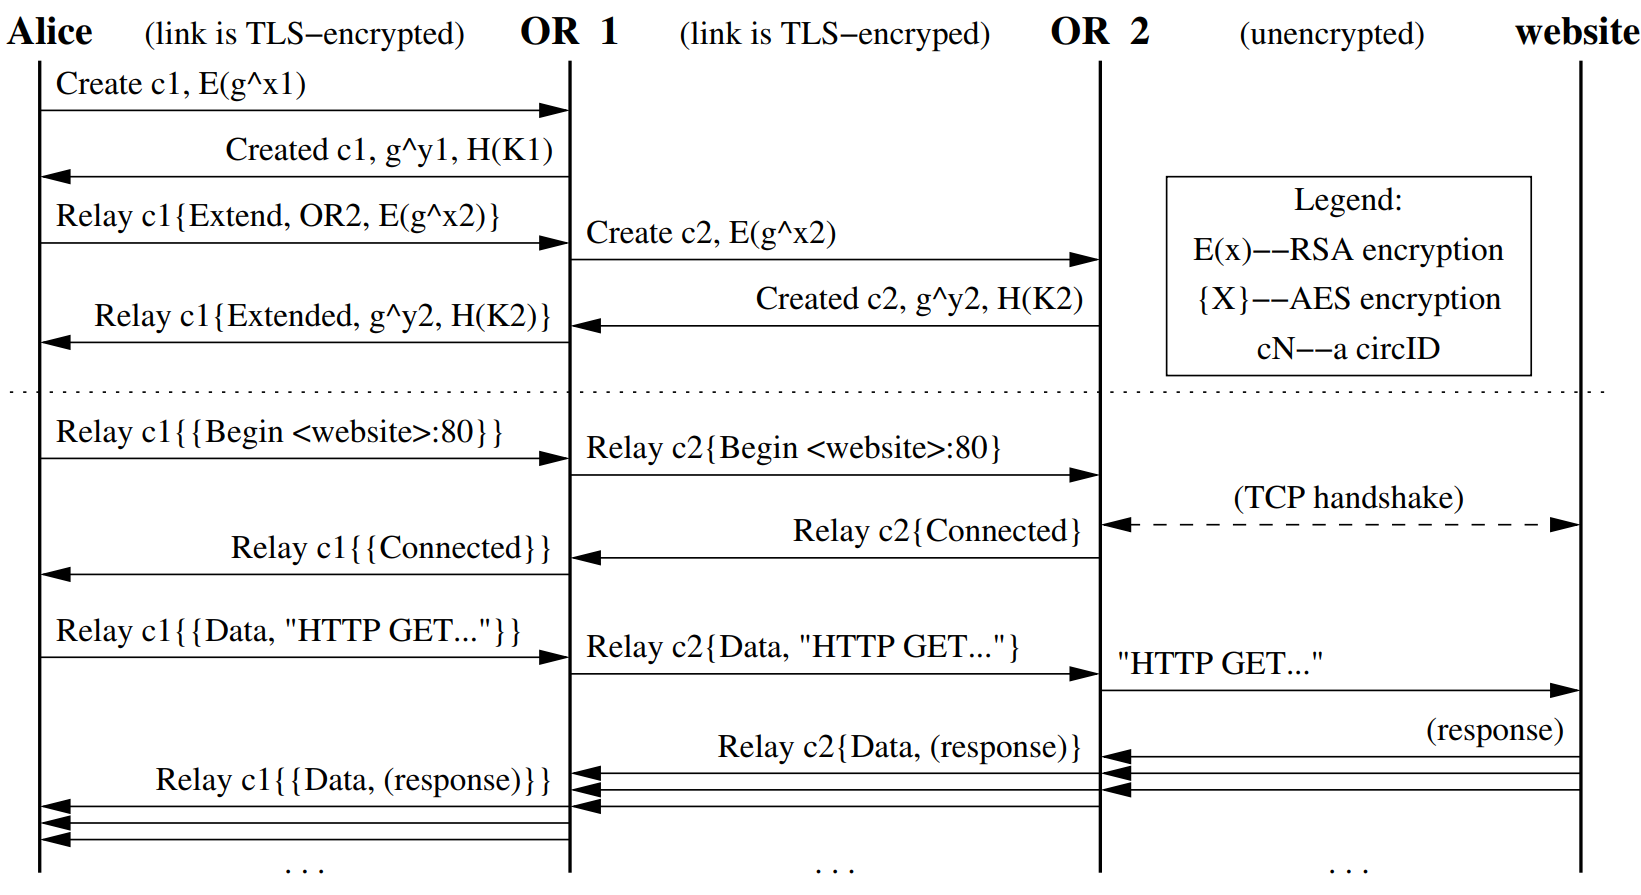
\includegraphics[width=\textwidth]{OR5.png}
  \caption{Diagrama representando un ejemplo de comunicación entre una usuaria (Alice) y una página web, pasando por dos nodos intermedios \parencite{dingledine_tor:_2004}.}
  \label{fig:or5}
\end{figure}

Puesto que solo el primer nodo conoce desde dónde proviene la información y sólo el nodo final conoce cuál es la información, no es posible saber quién la envía y qué se envía.

\section{Algoritmos de cifrado}
\label{sec:algoritmos}
% Jose

Como ya hemos comentado, las conexiones entre dos repetidores en un circuito Tor, o entre el cliente y un repetidor utilizan el protocolo TLS/SSLv3 para la autentificación y el cifrado de los enlaces.
Se conoce como \textit{suite de cifrado} al conjunto de algoritmos utilizados al realizar una comunicación mediante TLS.
Dicha \textit{suite} suele incluir un algoritmo de intercambio de intercambio de claves, un algoritmo de cifrado en bloque y un algoritmo de código de autentificación de mensaje.
Sin entrar en demasiados detalles, el protocolo TLS tiene dos fases: una primera en la que ambas partes establecen la conexión y se ponen de acuerdo en una clave compartida con la que cifrar la información (mediante el uso del algoritmo de intercambio de claves), y una segunda en la que proceden al intercambio de información en sí, utilizando para ello el algoritmo de cifrado en bloque \parencite{ibm_overview_2019}.

La especificación de Tor \parencite{dingledine_tor_2019} permite que el usuario elija una \textit{suite} de cifrado de entre una lista predefinida, aunque todas las disponibles son variaciones de la que que todas las implementaciones  de Tor deben soportar como mínimo, denominada \texttt{TLS\_DHE\_RSA\_WITH\_AES\_128\_CBC\_SHA}.
De esta forma, para llevar a cabo la primera fase del protocolo TLS, en la que se establece la conexión entre los nodos del circuito creado por el usuario, Tor utiliza una implementación del protocolo de Diffie-Hellman.
Originalmente Tor utilizaba un protocolo de autentificación ---denominado posteriormente como TAP, \textit{Tor Authentication Protocol}--- que implementaba la versión clásica de Diffie-Hellman sobre un grupo finito de orden primo junto a RSA para calcular el conjunto de claves que ambos nodos comparten \parencite{dingledine_tor:_2004}.
Análisis posteriores \parencite{hutchison_security_2006} llegaron a la conclusión de que TAP tenía deficiencias, debido a que hacía implementaciones no estándares de dichos protocolos. Esto condujo a la creación de un nuevo protocolo denominado \textit{ntor} y que se introdujo en la versión \texttt{0.2.4.8-alpha} de Tor.
Este nuevo protocolo utiliza ECDH (\textit{Elliptic Curve Diffie-Hellman}), que implementa el protocolo de Diffie-Hellman para un grupo de curvas elípticas, en lugar de un grupo finito de orden primo. Tor en concreto utiliza el grupo generado sobre la curva Curve25519, que ofrece seguridad de 128 bits \parencite{yung_curve25519:_2006}. Esto quiere decir que para romper dicho cifrado serían necesarias aproximadamente \(2^{128}\) operaciones.

Finalmente, una vez establecida la conexión TLS, se utiliza AES con claves de 128 bits para el cifrado de la información intercambiada entre dos nodos. En caso de que sea necesario el cálculo de algún \textit{hash}, se utiliza SHA-1 por defecto, aunque también se utilizan SHA256 y SHA3-256 en algunos puntos.

\subsection{Parámetros de los algoritmos}

La especificación de Tor describe los parámetros que se utilizan por defecto cuando se usa alguno de los algoritmos de cifrado descritos anteriormente, a saber: \begin{itemize}
  \item Para Diffie-Hellman sobre \(Z_p\) se utiliza como generador \(g=2\) y \(p\) es el primo seguro de 1024 bits descrito en \parencite{carrel_internet_1998}, cuyo valor es \[
    2^{1024} - 2^{960} - 1 + 2^{64} \cdot \left\lfloor (2^{894} \pi) + 129093 \right\rfloor.
  \]
  %y cuya representación hexadecimal se describe en la figura \ref{verb:primo-seguro}.
  % \begin{figure}[h]
  %   \centering
  %   \begin{BVerbatim}
  % FFFFFFFF FFFFFFFF C90FDAA2 2168C234 C4C6628B
  % 80DC1CD1 29024E08 8A67CC74 020BBEA6 3B139B22
  % 514A0879 8E3404DD EF9519B3 CD3A431B 302B0A6D
  % F25F1437 4FE1356D 6D51C245 E485B576 625E7EC6
  % F44C42E9 A637ED6B 0BFF5CB6 F406B7ED EE386BFB
  % 5A899FA5 AE9F2411 7C4B1FE6 49286651 ECE65381
  % FFFFFFFF FFFFFFFF
  %   \end{BVerbatim}
  %   \caption{Representación hexadecimal del primo}
  %   \label{verb:primo-seguro}
  % \end{figure}
  \item Para Diffie-Hellman con curvas elípticas se utiliza el grupo generado sobre la curva Curve25519, como ya se ha mencionado antes. Esta curva viene descrita por la ecuación \[
    y^{2}=x^{3}+486662x^{2}+x
  \]
  y se utiliza sobre el cuerpo finito de orden el primo \(2^{255}-19\).
  \item Para RSA se utilizan claves de tamaño \(1024\) y un exponente fijo, \(65537\), común en el cifrado mediante RSA.
\end{itemize}

\section{Posibles ataques}
\label{sec:ataques}
% Dani

\subsection{Modelo de amenazas}

Los modelos de amenazas más empleados en redes de anonimato son el del atacante
\emph{pasivo}, que puede observar el tráfico que llega a varios, o todos los
nodos de la red; y el del atacante \emph{activo}, que además puede participar en
la red.

El objetivo de este atacante será romper el anonimato de la red, es decir,
determinar las conexiones que se producen a través de ella.

El modelo de amenazas de Tor, en concreto, contempla atacantes que pueden
observar una parte del tráfico de la red ---pero no todo---; que puede generar,
modificar y retrasar tráfico, y participar en la red operando nodos, o
controlando nodos de confianza en la red. Además, puede denegar el servicio
tanto a usuarios como a nodos.

\subsection{Ataques pasivos}

En esta sección se asume el atacante pasivo, que puede observar el tráfico
mínimo necesario para realizar cada ataque.

\subsubsection{Ataques de correlación} \label{corrat}

Se trata de ataques en los que el atacante puede observar el tráfico que llega a
un nodo de entrada y a un servicio, y tratará de confirmar si el nodo de entrada
y el servicio participan en un circuito observando la relación estadística entre
el tráfico que llega al nodo de entrada y el que llega al servicio. Se puede
observar la correlación en el \emph{tiempo} en el que transcurre el tráfico y en
el \emph{tamaño} de dicho tráfico.

\subsubsection{Identificación mediante huellas digitales}

Un atacante puede compilar una base de datos de «huellas digitales»: patrones de
tráfico que caracterizan el acceso a ciertos servicios, y confirmar el acceso de
un usuario a un servicio buscando en la base de datos.

\subsection{Ataques activos}

\subsubsection{Reemplazo de contenidos en protocolos no autenticados}

Si un atacante controla un nodo de salida, y el tráfico que le llega corresponde
a una petición de un protocolo que no usa autenticación, puede devolver una
respuesta arbitraria, que sirva para identificar un nodo de entrada.

\subsubsection{Administrar nodos hostiles}

Si un atacante puede administrar $m$ nodos en una red de $N$ nodos,
$\left(\frac{m}{N}\right)^2$ de las veces un usuario elegirá dos nodos hostiles
como nodos de entrada y de salida, permitiendo la identificación de la conexión,
al estar los circuitos formados por tres nodos y conocer cada nodo el que le
precede y el que le sucede.

\subsubsection{Retrasar tráfico}

Un atacante puede introducir retrasos artificiales en el tráfico de la red para
apoyar un ataque de correlación como el descrito en \ref{corrat}.

%-------------------------------------------------------------------------------
%	BIBLIOGRAFÍA
%-------------------------------------------------------------------------------

\newpage
\printbibliography

\end{document}
